% Suggested update of the AALC results section (Section "Combined IPC Trailing Edge Flap Control
% Design and Application", \subsection{Results}, label subsec:ResultsTEF) in
% 04_WindTurbineControl_02_notBold.tex. Replaces that subsection up to the start of
% \subsection{Comparison of Wind Turbine Control Designs}; it uses the same labels, so it is meant
% to be \input instead of the existing subsection, not in addition to it.
% Changes to the existing text:
% - open-loop part unchanged
% - PSD figure: 18 m/s (optimization wind speed, optimization set, NTM class A, IPC/TEF fade-in,
%   8 deg/s) instead of 16 m/s, figures/figIPCThesis/fig02_PSDroot_breaky*_AALC*.eps
% - AALC gains of the current optimization (K_P,IPC = 0.082, K_I,IPC = 0.669, K_P,TEFC = 0.641)
% - table tabone replaced by figures/figIPCThesis/tab_AALC_summary.tex (makeAALC_SummaryTable in
%   the Combined-IPC-TEFC repository): wind speed ranges, no tower top DEL, C_Act = actuator power (Eq. CAct_calc)
\subsection{Results} \label{subsec:ResultsTEF}
This section discusses both open loop results, obtained with the simulation set-up depicted in Figure~\ref{fig:OLdiag}, as well as closed loop results, simulated with the control loop from Figure~\ref{fig:CLdiag}. Figure~\ref{fig:OLval} shows the steady state values, at three different TEF angles, of power $P_g$, rotor speed $\omega_r$, rotor thrust $T_r$, and blade pitch angle $\beta_{0}$ for all 14 wind speeds. Simulations at constant wind speeds are run for 660\,s to confirm the validity of the TEF model. Data from the initial 60\,s are excluded to avoid non-physical initialization artifacts and the mean values are calculated for each wind speed.
\begin{figure} [h]
\subfloat[Power and rotor speed]{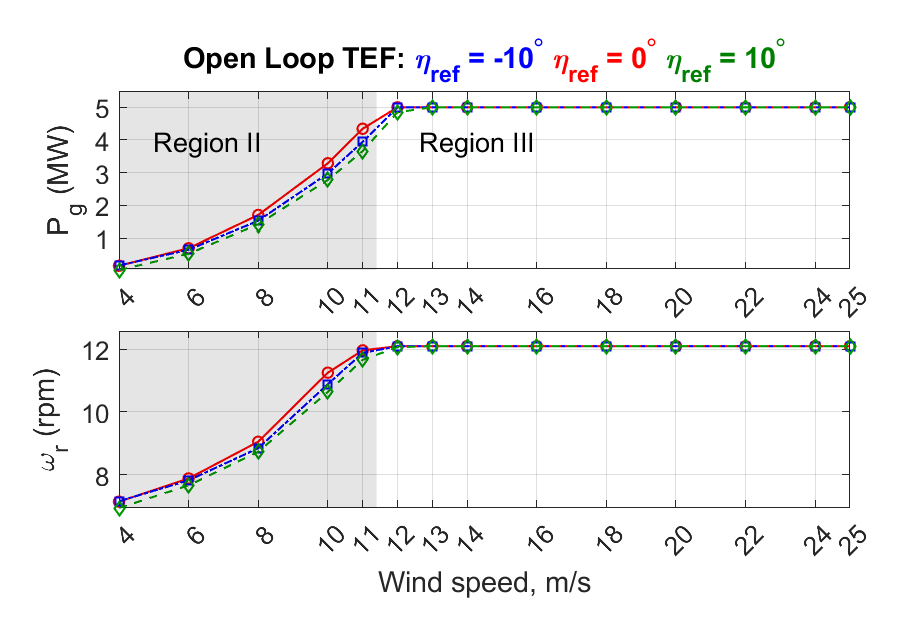
\includegraphics[width=0.485\textwidth]{figures/Images_Torque24/fig06_TEFOL_1.eps}}\hfill
\subfloat[Rotor thrust and blade pitch]{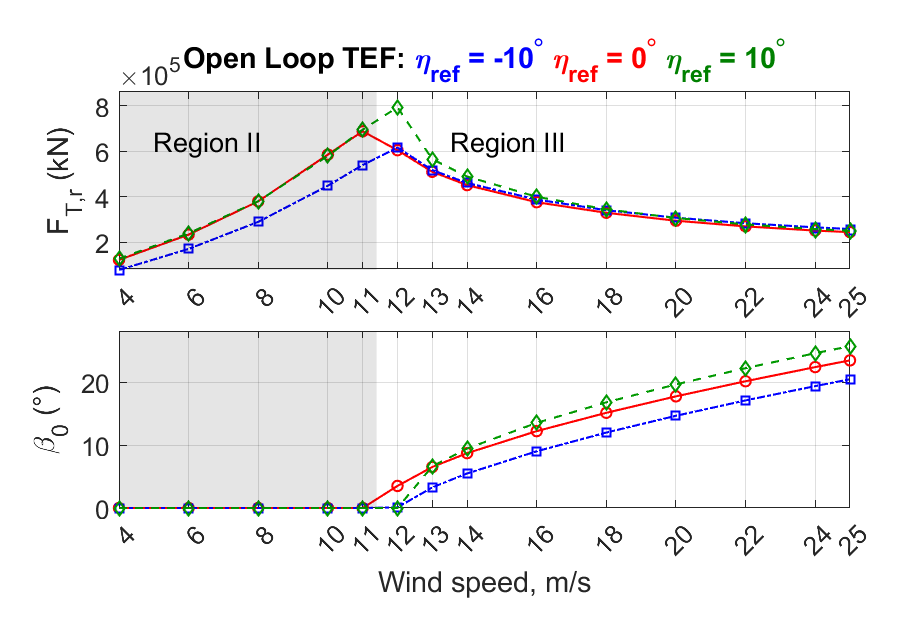
\includegraphics[width=0.485\textwidth]{figures/Images_Torque24/fig06_TEFOL_2.eps}}\hfill
\caption{TEF open-loop verification, TEF deflection at -10\textdegree{}\,(blue), 0\textdegree{}\,(red), and 10\textdegree{}\,(green).}
\label{fig:OLval}
\end{figure}

%
The simulated power with and without TEF deflections shows the expected power characteristic curve of a wind turbine: In Region~II, both positive and negative flap deflections reduce power \(P_g\) due to decreased aerodynamic efficiency, unlike in Region~III, where the same power output is observed, as the power controller controls the pitch angle once rated wind speed is reached. Adjusting the pitch changes the aerodynamic forces. The control system can therefore maintain nominal power. This also reflects on the rotor speed \(\omega_r\), depicted in the second plot, which is slightly lower in Region~II but unchanged in Region~III. The thrust \(T_r\) in Region~II is decreased by a negative flap angle, while the influence of a positive flap angle on the thrust is negligible: The thrust cannot be increased beyond the neutral flap position due to the limited wind power, which necessarily limits the amount of energy converted into rotational energy. This leads to a dynamic equilibrium where, despite positive flap deflection, the thrust forces remain at levels equivalent to those at the neutral flap position. The second plot in Figure~\ref{fig:OLval}\,(b) shows the blade pitch \(\beta_{0}\), which is lower for a negative and higher for a positive TEF angle, corresponding to the lower and higher thrust force.

Figure~\ref{fig:PSDTEF} shows the power spectral density (PSD) of the blade root bending moment in closed loop for the optimization dataset with a mean wind speed of 18\,m/s, the wind speed at which the AALC parameters are optimized.
\begin{figure} [h]
    \subfloat[Baseline (black), IPC (blue), and TEFC (green)]{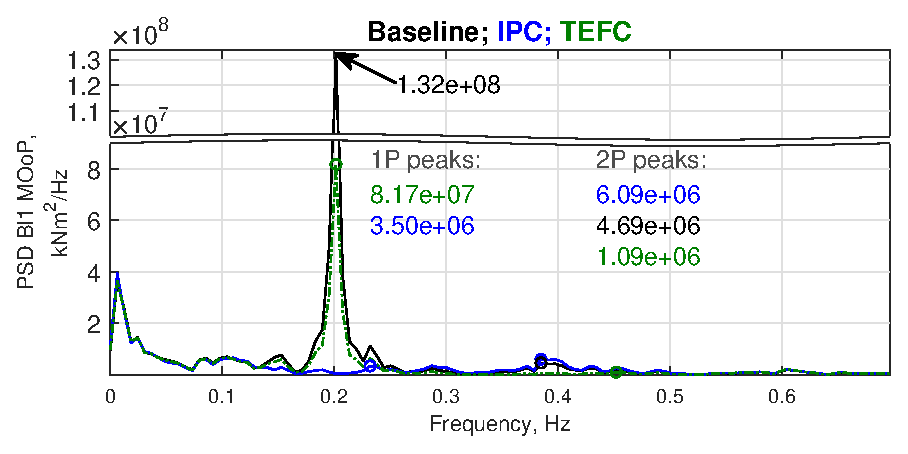
\includegraphics[width=0.485\textwidth]{figures/figIPCThesis/fig02_PSDroot_breaky_AALCinit.eps}}\hfill
    \subfloat[AALC (red), and AALC optimized (pink)]{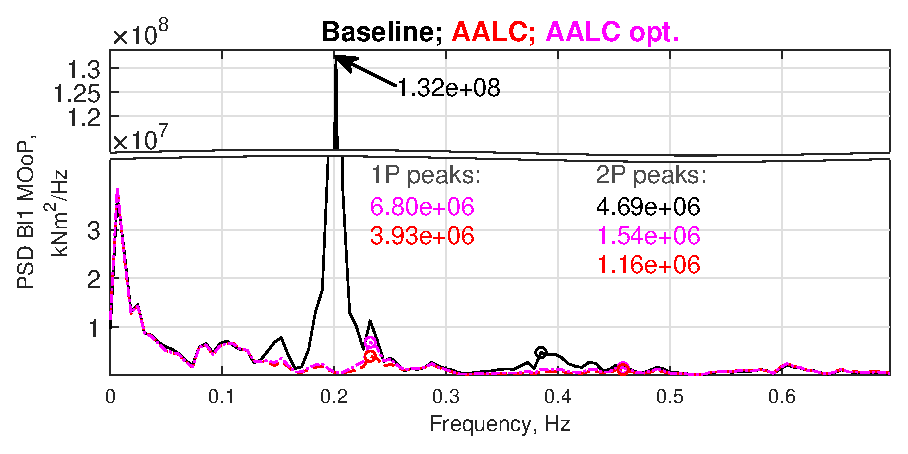
\includegraphics[width=0.485\textwidth]{figures/figIPCThesis/fig02_PSDroot_breaky1c_AALC.eps}}\hfill
    \caption{Power Spectral Density of the blade root out-of-plane moment for the optimization set, turbulence class A, with mean wind speed 18~m/s.}
    \label{fig:PSDTEF}
\end{figure}
%
IPC (blue line) and TEFC (green line) reduce the PSD of the 1P and 2P loads, respectively, compared to the baseline (black line): IPC alone reduces the 1P peak by 97.4\%, but increases the 2P peak by 29.8\%, while TEFC alone reduces the 2P peak by 76.8\% and the 1P peak by 38.3\%. These PSDs are obtained with the initially used AALC parameters with the original setting of a purely integral IPC and a purely proportional TEFC feedback, both set to values of one. In a second step, the three parameters \(K_{P,\text{IPC}}\), \(K_{I,\text{IPC}}\), and \(K_{P,\text{TEFC}}\) are optimized at 18\,m/s, subject to the constraint that the tower base DEL does not exceed the one of the baseline, resulting in an IPC PI controller with $K_{P,\text{IPC}} = 0.082$ and $K_{I,\text{IPC}} = 0.669$ and a TEFC P controller with $K_{P,\text{TEFC}} = 0.641$. An optimization started from the initial parameters instead of the optimized IPC parameters converges to the same cost.

Figure~\ref{fig:PSDTEF}\,(b) demonstrates that considerable improvement with respect to the baseline controller is possible using the suggested AALC design: The combined IPC-TEFC with the original setting of a purely integral IPC and proportional TEFC feedback reduces the PSD at 1P by 97.0\%, and at 2P by 75.3\%. With the optimized parameters, the reduction with respect to the baseline is 94.9\% at 1P and 67.3\% at 2P, i.e., the residual peaks are larger than with the initial setting. The cost function, the largest of the three blade DELs, is nevertheless decreased from $J = 0.778$ for the initial controller to $J = 0.773$ for the optimized one, as the optimized controller reduces the DELs of the three blades more evenly (by 22.7\% to 23.3\%, compared to 22.2\% to 25.1\% with the initial setting). At the same time, the optimized AALC requires less pitch activity than the optimized IPC without TEF: the standard deviation of the pitch rate is 2.14\textdegree/s compared to 2.98\textdegree/s.
From this study, it seems unlikely that a parameter optimization of the suggested, carefully designed controller can decrease the blade damage equivalent loads considerably. Further investigations might be made with respect to how much improvement is achievable with a more sophisticated MIMO controller.

Apart from the blade root flapwise moment, the influence of the obtained controller parameters is compared with respect to the evaluation criteria provided in Section~\ref{sec:ControllerParameterOptimization}.
Table~\ref{tabone} contains the five evaluation criteria to quantify the effect of the AALC: blade and tower base DEL, mean of generated power $\bar{P}_{g}$, its standard deviation $\sigma P$, and actuator power $C_{\text{Act}}$, Equation~\eqref{eq:CAct}, normalized by simulations without AALC for the same wind test cases. From 10\,m/s on, the parameters optimized at 18\,m/s are used. Below, the AALC parameters are scheduled with the parameters optimized separately at 4, 6, and 8\,m/s. The criteria are averaged over five wind speed ranges: all wind speeds, the wind speeds below and above rated, the wind speeds from 18\,m/s, and the optimization wind speed of 18\,m/s.
% Created by makeAALC_SummaryTable on 2026-10-25
\begin{table}[h]
    \centering
    \caption[Wind turbine evaluation criteria for AALC: Mean values of the optimization and verification datasets over wind speed ranges]{\label{tabone} Wind turbine evaluation criteria for AALC: Mean values of the optimization and verification datasets over different wind speed ranges, normalized by the baseline without AALC. From 10\,m/s on, the AALC gains optimized at 18\,m/s are used: $K_{P,\text{IPC}} = 0.082$, $K_{I,\text{IPC}} = 0.669$ and $K_{P,\text{TEFC}} = 0.641$; below, the gains are scheduled with the gains optimized at 4, 6 and 8\,m/s. Criteria are tower base and blade DELs, power mean and standard deviation (mean of the ratios of the single wind speeds), and the pitch activity (ratio of the mean pitch rates, since the baseline pitch is constant at low wind speeds; not given below rated, where the baseline pitch rate is close to zero). The first verification set has no wind fields for 11 and 13\,m/s.}
    \begin{tabular}{@{}l*{7}{c}@{}}
        \toprule
        Wind speeds & Dataset & Turb. class & $C_{\text{DEL},b}$ & $C_{\text{DEL},t,\text{Base}}$ & $C_{\bar{P}}$ & $C_{\delta P}$ & $C_{\text{Act}}$ \\
        \midrule
        \multirow{3}{*}{All (4--25\,m/s)} & Optim. & A & 0.78 & 0.97 & 0.99 & 1.01 & 4.77 \\
         & Verif. 1 & A & 0.86 & 0.98 & 0.99 & 1.00 & 5.04 \\
         & Verif. 2 & B & 0.81 & 0.99 & 0.99 & 1.00 & 4.93 \\
        \midrule
        \multirow{3}{*}{Below rated (4--11\,m/s)} & Optim. & A & 0.81 & 0.94 & 0.98 & 1.00 & -- \\
         & Verif. 1 & A & 0.97 & 0.93 & 0.97 & 0.98 & -- \\
         & Verif. 2 & B & 0.85 & 0.96 & 0.98 & 0.98 & -- \\
        \midrule
        \multirow{3}{*}{Above rated (12--25\,m/s)} & Optim. & A & 0.77 & 0.99 & 1.00 & 1.02 & 3.67 \\
         & Verif. 1 & A & 0.81 & 1.00 & 1.00 & 1.01 & 3.74 \\
         & Verif. 2 & B & 0.79 & 1.00 & 1.00 & 1.02 & 3.77 \\
        \midrule
        \multirow{3}{*}{18--25\,m/s} & Optim. & A & 0.75 & 1.00 & 1.00 & 1.00 & 3.95 \\
         & Verif. 1 & A & 0.78 & 1.00 & 1.00 & 1.00 & 3.83 \\
         & Verif. 2 & B & 0.74 & 1.01 & 1.00 & 1.00 & 4.05 \\
        \midrule
        \multirow{3}{*}{18\,m/s} & Optim. & A & 0.77 & 0.99 & 1.00 & 0.99 & 3.66 \\
         & Verif. 1 & A & 0.82 & 1.00 & 1.00 & 1.00 & 3.44 \\
         & Verif. 2 & B & 0.78 & 1.03 & 1.00 & 1.00 & 3.59 \\
        \bottomrule
    \end{tabular}
\end{table}


Above rated, the blade DEL decreases by 19\% to 23\%, and from 18\,m/s on by 22\% to 26\%, with the largest reduction for the second verification set of turbulence class~B. The parameters optimized at a single wind speed hence carry over to the whole of Region~III and to both verification sets, so that no gain scheduling is required above rated. The tower base DEL is not changed considerably above rated, with criteria between 0.99 and 1.00; the largest increase of a single wind speed is 3\% at 18\,m/s for turbulence class~B. Below rated, the blade DEL is reduced by 19\% for the optimization set and by 15\% for the second verification set, but only by 3\% for the first verification set, i.e., the parameters optimized below rated do not carry over reliably to other wind fields. Here, the tower base DEL is reduced by 4\% to 7\%. Including all wind speeds, the blade DEL is reduced by 14\% to 22\%.

 The evaluation of the power criteria confirms that the AALC leads only to negligible changes in both power mean and variance above rated. Below rated, the mean power is decreased by 2\% to 3\%, as the flap and pitch deflections reduce the aerodynamic efficiency, cf.\ Figure~\ref{fig:OLval}. The additional rotational movement of the blade demanded by IPC is the only criterion leading to an unavoidable increase, similar to the two controller schemes discussed in previous sections: above rated, the actuator power is increased by a factor of 3.8 to 4.0, and from 18\,m/s on by a factor of 3.9 to 4.2. Below rated, the baseline pitch angle is almost constant, so that the baseline actuator power is close to zero and no meaningful ratio is obtained. To assess the overall performance of AALC relative to the other discussed control strategies, the following section presents a comparison of all three investigated algorithms on load reduction and  power standard deviation at different pitch rate limits.
